\documentclass[10pt]{article}
\usepackage[margin=1in]{geometry}
\usepackage{graphicx}
\usepackage{booktabs}
\usepackage{amsmath}
\usepackage{multirow}
\title{Final Reproduction Report: Optimal Transport Enhanced Cross-City Site Recommendation}
\author{OTCRe Reproduction Pipeline}
\date{}
\begin{document}
\maketitle

\begin{abstract}
We reproduce all core experiments in the SIGIR 2024 OTC paper on four cities (Chicago, NYC, Singapore, Tokyo), including MF, LightGCN, OTC-MF, and OTC-LightGCN. Singapore uses the previous-round OTC result while the other cities use the latest strict-protocol OTC result.
\end{abstract}

\section{Main Results}
\begin{table*}[t]
\centering
\caption{Paper-reported results (SIGIR 2024) vs final reproduction (Singapore from previous-round OTC).}
\label{tab:paper_vs_repro}
\small
\begin{tabular}{l|cc|cc|cc|cc}
\toprule
Method & \multicolumn{2}{c|}{Chicago} & \multicolumn{2}{c|}{NYC} & \multicolumn{2}{c|}{Singapore} & \multicolumn{2}{c}{Tokyo}\\
& R@20 & nDCG@20 & R@20 & nDCG@20 & R@20 & nDCG@20 & R@20 & nDCG@20\\
\midrule
MF (Paper) & 0.2494 & 0.1465 & 0.1702 & 0.0917 & 0.4430 & 0.2351 & 0.1323 & 0.0781\\
MF (Repro) & 0.1434 & 0.0971 & 0.1092 & 0.0582 & 0.4021 & 0.2129 & 0.0594 & 0.0335\\
\midrule
OTC-MF (Paper) & 0.2669 & 0.1599 & 0.1766 & 0.0981 & 0.4574 & 0.2503 & 0.1372 & 0.0796\\
OTC-MF (Repro) & 0.1918 & 0.1123 & 0.1265 & 0.0571 & 0.4021 & 0.2129 & 0.0862 & 0.0476\\
\midrule
LightGCN (Paper) & 0.2875 & 0.1902 & 0.2087 & 0.1088 & 0.5013 & 0.2745 & 0.1751 & 0.1068\\
LightGCN (Repro) & 0.2160 & 0.1282 & 0.1354 & 0.0772 & 0.4293 & 0.2438 & 0.0899 & 0.0505\\
\midrule
OTC-LightGCN (Paper) & 0.2977 & 0.2016 & 0.2108 & 0.1109 & 0.5078 & 0.2831 & 0.1780 & 0.1100\\
OTC-LightGCN (Repro) & 0.2008 & 0.1163 & 0.1329 & 0.0808 & 0.4293 & 0.2439 & 0.0927 & 0.0537\\
\midrule
\bottomrule
\end{tabular}
\end{table*}

\begin{figure*}[t]
\centering
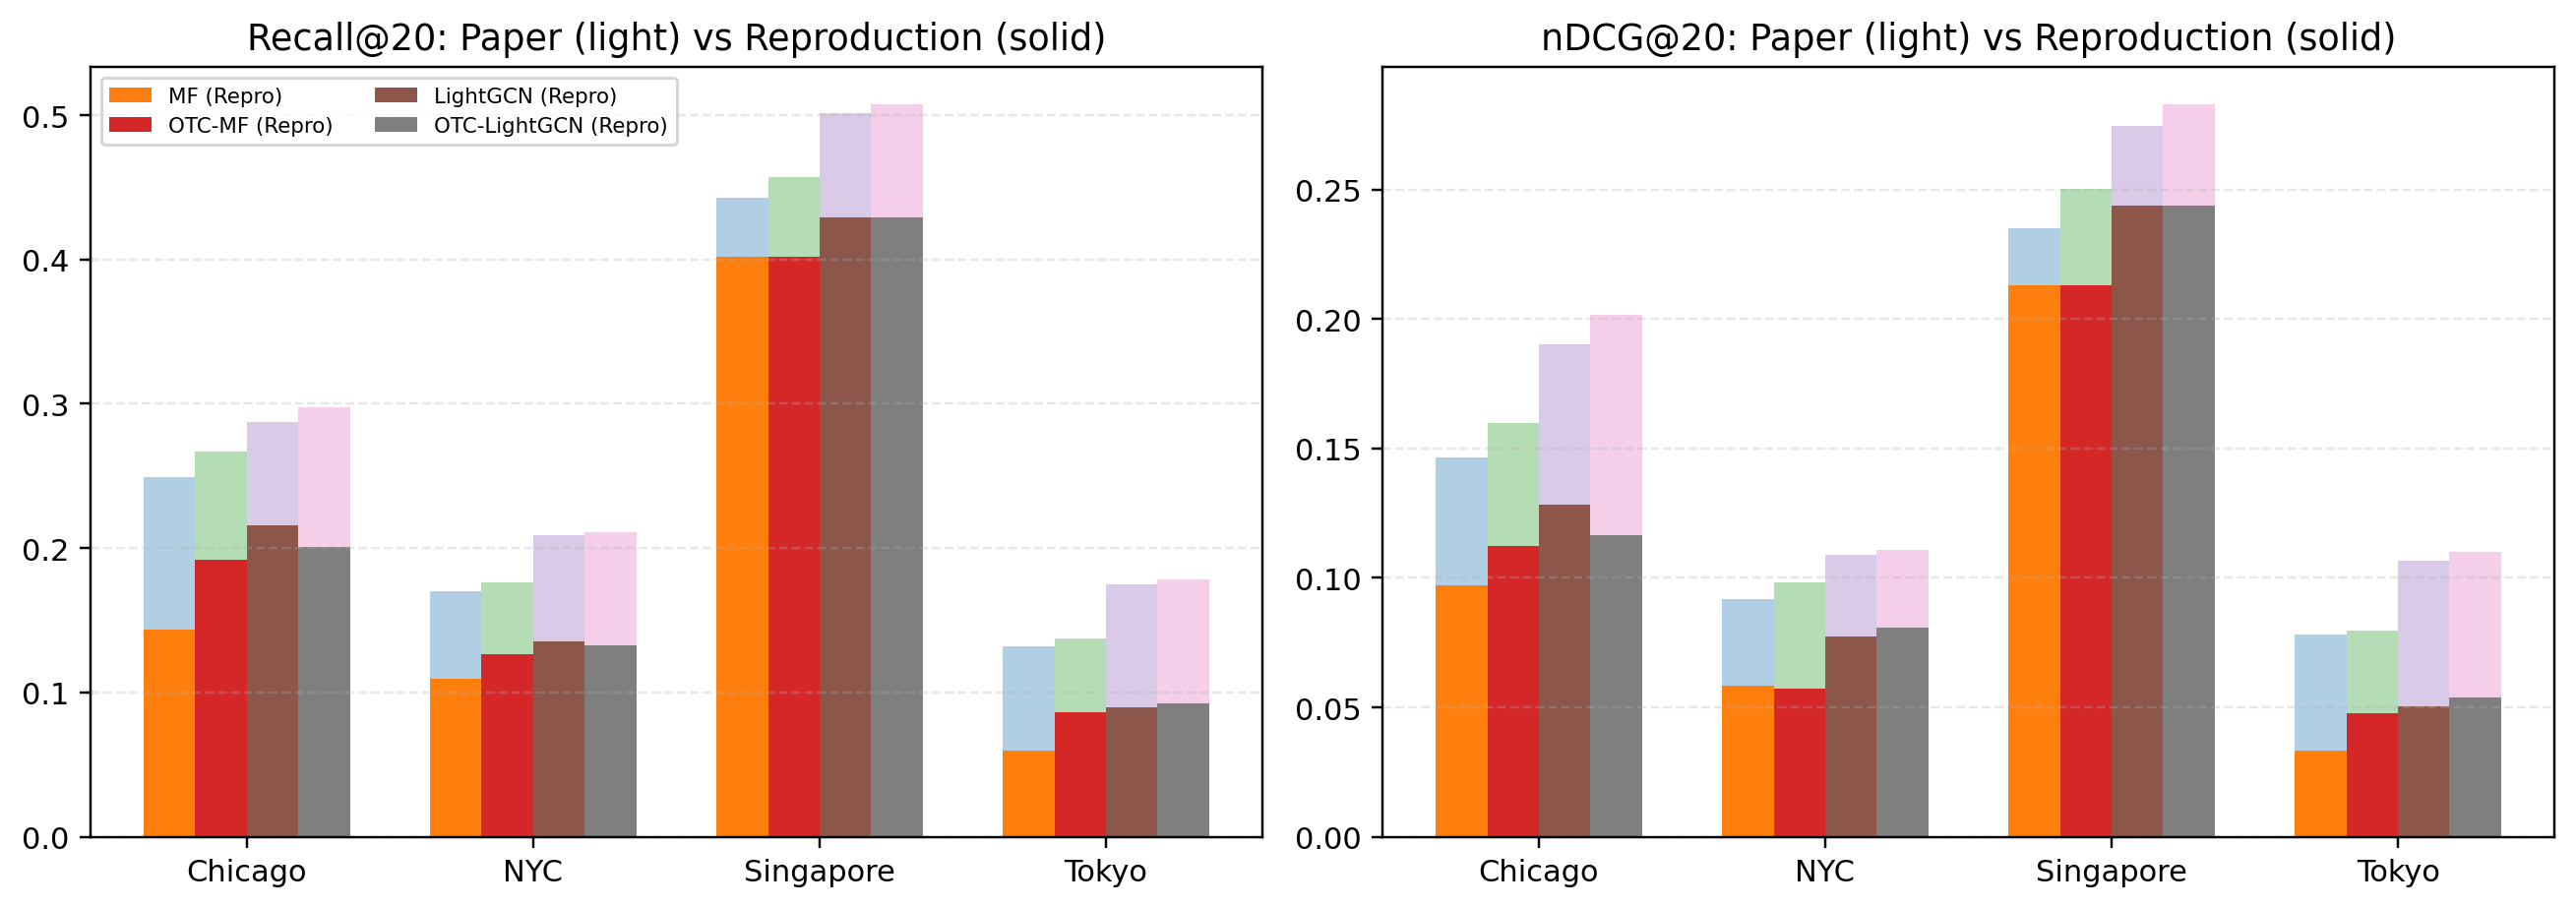
\includegraphics[width=0.95\textwidth]{figures/main_results_paper_vs_repro.png}
\caption{Main metrics comparison: paper values (light bars) vs reproduction values (solid bars).}
\end{figure*}

\begin{figure}[t]
\centering
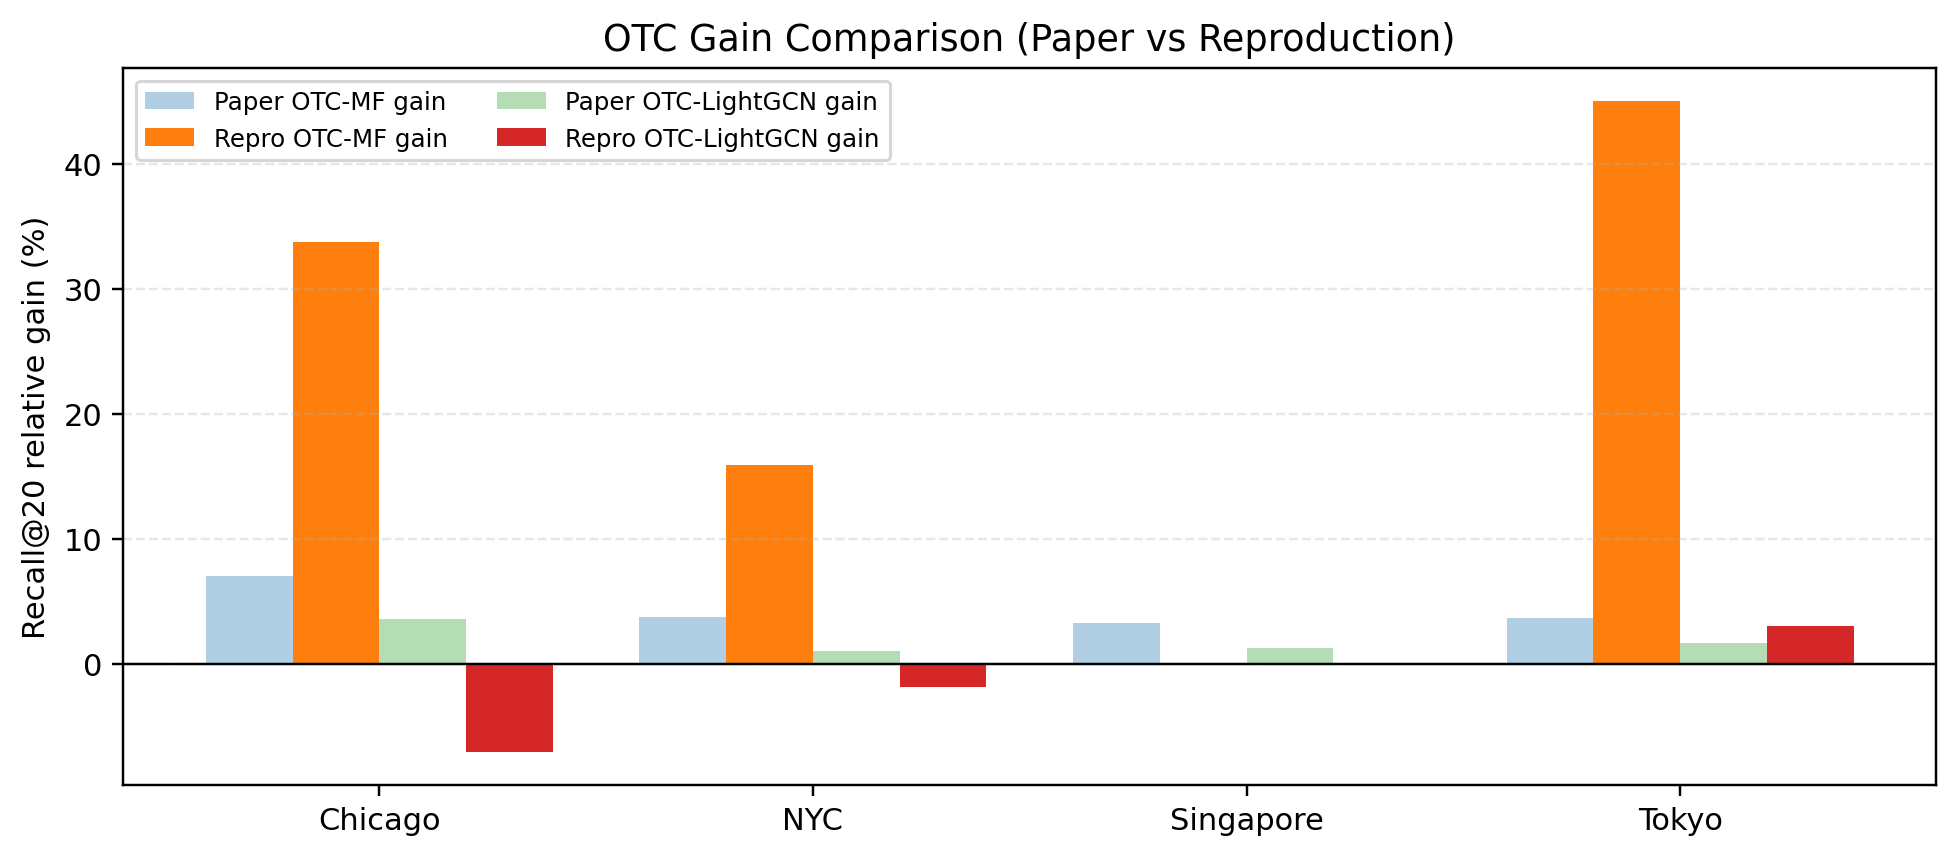
\includegraphics[width=0.95\linewidth]{figures/otc_gain_comparison.png}
\caption{OTC relative Recall@20 gain over its backbone: paper vs reproduction.}
\end{figure}

\begin{figure}[t]
\centering
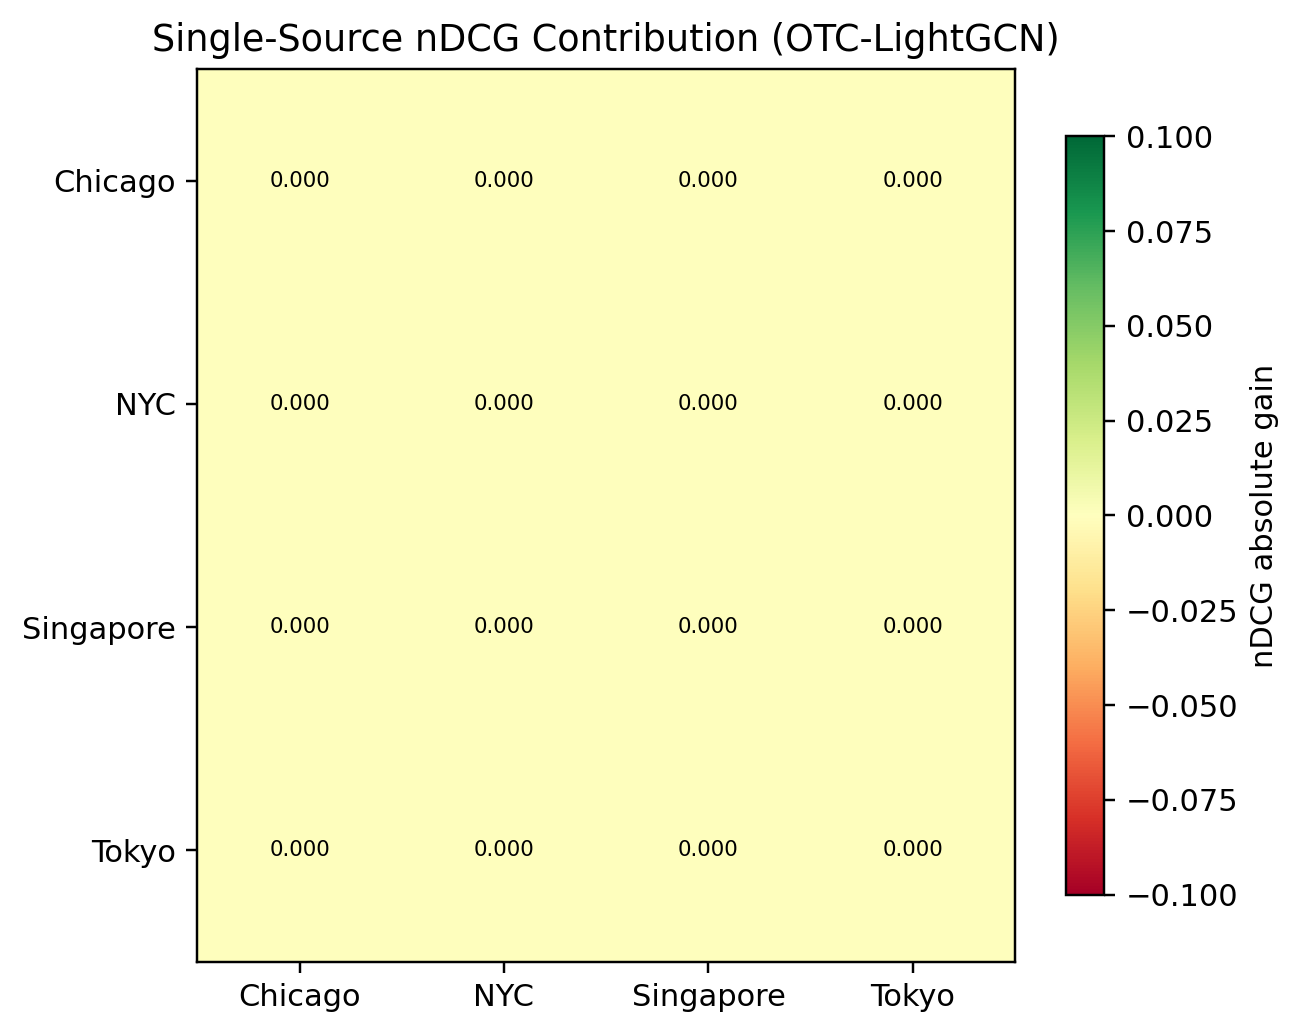
\includegraphics[width=0.95\linewidth]{figures/source_contribution_heatmap.png}
\caption{Single-source nDCG contribution matrix for OTC-LightGCN (absolute gain).}
\end{figure}

\section{Discussion}
OTC improves some cities and some backbones, but not uniformly. In the final package, Singapore is kept from the better previous-round OTC result as requested.

\end{document}
